%!TEX root = ../template.tex
%%%%%%%%%%%%%%%%%%%%%%%%%%%%%%%%%%%%%%%%%%%%%%%%%%%%%%%%%%%%%%%%%%%%
%% chapter4.tex
%% NOVA thesis document file
%%
%% Chapter with lots of dummy text
%%%%%%%%%%%%%%%%%%%%%%%%%%%%%%%%%%%%%%%%%%%%%%%%%%%%%%%%%%%%%%%%%%%%
\chapter{Resultados}
\label{cha:Resultados}

En la topología de dos routers, correspondiente al diseño de las sedes nacionales se observó que el diseño realizado garantiza la conectividad hacia el centro de datos, y dependiendo de la aplicación que se utilice el tráfico será enrutado por una última milla o por la otra, las imágenes  \textbf{Ver figura 11.1 Conectividad} y  \textbf{Ver figura 11.2  Ruta} muestran esta conectividad y la ruta que se está tomando para dicho tráfico. 

\begin{figure}[htbp]
  \centering
  %\subcaptionbox{\label{fig:leftsubfig}}%
    {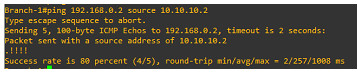
\includegraphics[width=0.5\linewidth]{figure56}}%
%  \subcaptionbox{Another sub-figure\label{fig:rightsubfig}}%
%    {
\includegraphics[width=0.5\linewidth]{knitting-vectorial}}%
  \caption{ \footnotesize{Conectividad}}
  \footnotesize{\textbf{Tomado de:} \textit{autores}.}
  \label{fig:fig2subfig}
\end{figure}

\begin{figure}[htbp]
  \centering
  %\subcaptionbox{\label{fig:leftsubfig}}%
    {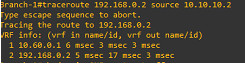
\includegraphics[width=0.5\linewidth]{figure57}}%
%  \subcaptionbox{Another sub-figure\label{fig:rightsubfig}}%
%    {
\includegraphics[width=0.5\linewidth]{knitting-vectorial}}%
  \caption{\footnotesize{ Ruta}}
  \footnotesize{\textbf{Tomado de:} \textit{autores}.}
  \label{fig:fig2subfig}
\end{figure}

El router reconoce mediante Nbar las aplicaciones que cursan por la red y dependiendo de esto y de los parámetros de retardo, jitter y pérdida de paquetes decide por cuál de las interfaces disponibles enviar el tráfico, en este caso el tráfico de ping fue enrutado a través de la MPLS como lo indica la figura \textbf{Ver figura 11.3 Enrutado a través de la MPLS}

\begin{figure}[htbp]
  \centering
  %\subcaptionbox{\label{fig:leftsubfig}}%
    {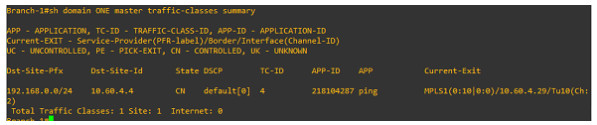
\includegraphics[width=0.6\linewidth]{figure58}}%
%  \subcaptionbox{Another sub-figure\label{fig:rightsubfig}}%
%    {
\includegraphics[width=0.5\linewidth]{knitting-vectorial}}%
  \caption{ \footnotesize{Enrutado a través de la MPLS}}
  \footnotesize{\textbf{Tomado de:} \textit{autores}.}
  \label{fig:fig2subfig}
\end{figure}

Posterior a realizar las pruebas de conectividad se quisieron medir los mecanismos de redundancia implementados y para ello se simuló la caída del enlace MPLS con el fin de verificar que se cumpla la alta disponibilidad deseada en la red.


\begin{figure}[htbp]
  \centering
  %\subcaptionbox{\label{fig:leftsubfig}}%
    {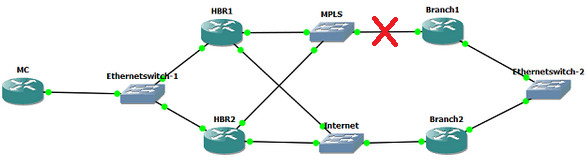
\includegraphics[width=0.6\linewidth]{figure59}}%
%  \subcaptionbox{Another sub-figure\label{fig:rightsubfig}}%
%    {
\includegraphics[width=0.5\linewidth]{knitting-vectorial}}%
  \caption{\footnotesize{ Disponibilidad Deseada en la Red}}
  \footnotesize{\textbf{Tomado de:} \textit{autores}.}
  \label{fig:fig2subfig}
\end{figure}

Al simular una ruptura de fibra sobre la MPLS el tráfico conmutó al enlace de internet y ya que PfR mide pérdidas de paquetes en los túneles toda la solución de IWAN conmutó hacia el único enlace disponible. La figura \textbf{Ver figura 11.4 Disponibilidad Deseada en la Red} muestra como el tráfico ahora tomo otro camino para llegar al mismo destino y la figura \textbf{Ver figura 11.5 Reconocimiento del cambio en PfR} ilustra el reconocimiento del cambio en PfR y por tanto el cambio en las políticas de enrutamiento.
 
 \begin{figure}[htbp]
  \centering
  %\subcaptionbox{\label{fig:leftsubfig}}%
    {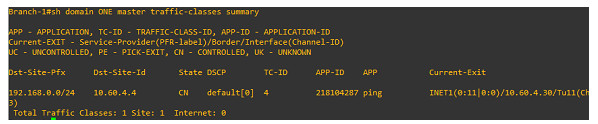
\includegraphics[width=0.6\linewidth]{figure60}}%
%  \subcaptionbox{Another sub-figure\label{fig:rightsubfig}}%
%    {
\includegraphics[width=0.5\linewidth]{knitting-vectorial}}%
  \caption{ \footnotesize{Reconocimiento del cambio en PfR}}
  \footnotesize{\textbf{Tomado de:} \textit{autores}.}
  \label{fig:fig2subfig}
\end{figure}

El mismo tipo de pruebas fueron realizadas sobre la topología de las sedes regionales, que cuentan con conexión a dos tipos de transporte diferentes pero un solo CPE en la sede, las pruebas de conectividad arrojaron exactamente los mismos resultados que en el escenario anterior, es decir conectividad exitosa a través de la MPLS como puede verse en la figura \textbf{Ver figura 11.6 Topología de las Sedes Regionales} y \textbf{Ver figura 11.7 Conectividad exitosa a través de la MPLS}

\begin{figure}[htbp]
  \centering
  %\subcaptionbox{\label{fig:leftsubfig}}%
    {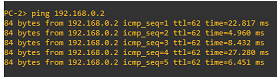
\includegraphics[width=0.5\linewidth]{figure61}}%
%  \subcaptionbox{Another sub-figure\label{fig:rightsubfig}}%
%    {
\includegraphics[width=0.5\linewidth]{knitting-vectorial}}%
  \caption{\footnotesize{ Topología de las Sedes Regionales}}
 \footnotesize{ \textbf{Tomado de:} \textit{autores}.}
  \label{fig:fig2subfig}
\end{figure}

\begin{figure}[htbp]
  \centering
  %\subcaptionbox{\label{fig:leftsubfig}}%
    {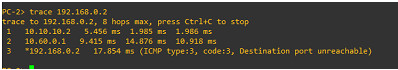
\includegraphics[width=0.6\linewidth]{figure62}}%
%  \subcaptionbox{Another sub-figure\label{fig:rightsubfig}}%
%    {
\includegraphics[width=0.5\linewidth]{knitting-vectorial}}%
  \caption{\footnotesize{Conectividad exitosa a través de la MPLS}}
 \footnotesize{ \textbf{Tomado de:} \textit{autores}.}
  \label{fig:fig2subfig}
\end{figure}

Al igual que en el escenario de dos router la aplicación es reconocida y enrutada a través de la MPLS según las políticas de PfR, por lo que se comprueba que tanto el reconocimiento de aplicaciones como el enrutamiento basado en aplicación se encuentra funcionando apropiadamente. La figura \textbf{Ver figura 11.8 Decisión de PfR} muestra la decisión de PfR de enrutar el tráfico ping a través de la MPLS.

\begin{figure}[htbp]
  \centering
  %\subcaptionbox{\label{fig:leftsubfig}}%
    {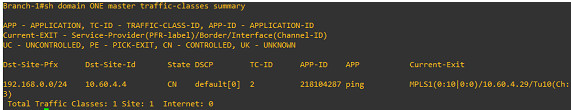
\includegraphics[width=0.6\linewidth]{figure63}}%
%  \subcaptionbox{Another sub-figure\label{fig:rightsubfig}}%
%    {
\includegraphics[width=0.5\linewidth]{knitting-vectorial}}%
  \caption{\footnotesize{Decisión de PfR}}
  \footnotesize{\textbf{Tomado de:} \textit{autores}.}
  \label{fig:fig2subfig}
\end{figure}

Al igual que como se realizó con el escenario de dos routers, se generaron pruebas de simulación de falla de fibra con el fin de comprobar que la redundancia de la operación funcione correctamente. La figura  \textbf{Ver figura 11.9 Falla de Fibra} se ilustra la prueba realizada para este escenario.

\begin{figure}[htbp]
  \centering
  %\subcaptionbox{\label{fig:leftsubfig}}%
    {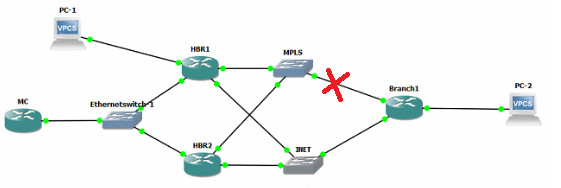
\includegraphics[width=0.6\linewidth]{figure64}}%
%  \subcaptionbox{Another sub-figure\label{fig:rightsubfig}}%
%    {
\includegraphics[width=0.5\linewidth]{knitting-vectorial}}%
  \caption{\footnotesize{Falla de Fibra }}
  \footnotesize{\textbf{Tomado de:} \textit{autores}.}
  \label{fig:fig2subfig}
\end{figure}

Después de simular esta falla se realizaron pruebas de conectividad exitosa \textbf{Ver figura 11.10 Enlace de INET}  y tal como lo indica la traza tomada,el tráfico conmutó correctamente a través del enlace de INET.


\begin{figure}[htbp]
  \centering
  %\subcaptionbox{\label{fig:leftsubfig}}%
    {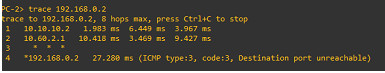
\includegraphics[width=0.6\linewidth]{figure65}}%
%  \subcaptionbox{Another sub-figure\label{fig:rightsubfig}}%
%    {
\includegraphics[width=0.5\linewidth]{knitting-vectorial}}%
  \caption{\footnotesize{Enlace de INET}}
  \footnotesize{\textbf{Tomado de:} \textit{autores}.}
  \label{fig:fig2subfig}
\end{figure}

Los resultados de la simulación muestran por tanto que el esquema de redundancia funciona apropiadamente ante una falla de un equipo o en el caso de ruptura de fibra, lo mismo aplica para casos de degradación de los servicios por pérdidas de paquetes o retardos excesivos en alguno de los transportes.